\documentclass[twocolumn]{aastex62}

\usepackage{stix}
\usepackage{xspace}
\usepackage{todonotes}
\newcommand{\vdag}{(v)^\dagger}
\newcommand\aastex{AAS\TeX}
\newcommand\latex{La\TeX}
\newcommand{\mjup}{\ensuremath{M_\mathrm{Jup}}\xspace}
\newcommand{\teff}{\ensuremath{T_{\mathrm{eff}}}\xspace}
\graphicspath{{./}{figures/}}
\shorttitle{HD106906b Time Resolved Observations}
\shortauthors{Zhou et al.}

\begin{document}


\title{Cloud Atlas: High-precision time-resolved observations of exoplanet HD106906b}

\correspondingauthor{Yifan Zhou}
\email{yzhou@as.arizona.edu}

\author{Yifan Zhou}
\affil{Steward Observatory}

\author{D\'aniel Apai}
\affil{Steward Observatory}

\begin{abstract}
  This documents keep the main result for \emph{Cloud Atlas} HD106906b \citep{Bailey2013} observations.
\end{abstract}

\keywords{}
\listoftodos

\section{Introduction}

HD106906b, a $11\pm2$ \mjup  mass exoplanet \citep{Bailey2013}, and its host, a F5V type star, form a peculiar system. This system, at a distance of $103.3\pm0.4$ pc \citep{Gaia2016,Gaia2018}, is a member of the Lower Centaurus Crux association (99.8 membership probability based on estimation from BANYAN-$\Sigma$, \citealt{Gagne2018} ), and a part of the Sco-Cen star forming region \citep[average age: $15\pm3$ Myr][]{Pecaut2016}. The planet and the star has a wide angular separation of $7\arcsec.11\pm0\arcsec.03$ corresponding to a projected distance of $734\pm4$ au. The planetary mass, ultra-cool atmosphere, and large angular separation place HD106906b as a prime target for exoplanet atmospheric studies \citep{Bailey2013,Kalas2015,Wu2016,Daemgen2017}. This young system also provides a critical test case for planet formation theories.

Multi-wavelength photometry \citep{Bailey2013,Kalas2015,Wu2016} and spectroscopy \citep{Daemgen2017} observations have been used to characterize the atmosphere of HD106906b.  These studies agree on an effective temperature (\teff) of 1800~K or a spectral type of L2.5-3. Based on the triangle-shaped of the $H$-band spectrum, \citet{Bailey2013, Daemgen2017} classified HD106906b as a intermediate- to low-surface gravity object. The low surface gravity classification is also consistent with the young age of the system. Like many other young L-type planetary mass companion (AB Pic B, 2M1207b, HR8799bcde), HD106906b appears redder than field brown dwarfs for its nIR color on the $M_{J}$-$J-K$ color magnitude diagram. The reddened nIR color is often associated with dusty atmospheres and thick condensate clouds \citep[e.g.,][]{Skemer2011}. Heterogeneous condensate clouds have been proved for causing rotational modulations in the nIR light curves of planetary mass objects \citep[e.g.,][]{Zhou2016,Vos2017,Biller2017,Biller2015,Lew2016,Manjavacas2017,Zhou2019}. High-precision nIR time-series observations will be able to reveal the cloud structures for HD106906b.

The formation pathway of HD106906b remains unclear. Disk fragmentation can hardly form a planet/companion with mass as small as that of HD106906b \citep[e.g.,][]{Kratter2010}. At a distance of more than 700~au from its host star, HD106906b cannot accrete enough material through \emph{in situ} core accretion. Furthermore, the current location of HD106906b significantly deviates from the circumstellar disk \citep{Bailey2013,Kalas2015}, which argues against \emph{in situ} core accretion but for that the planet orbit has experienced dynamical evolution during the planet's formation and evolution history. \citep{DeRosa2019} discovered a close near-coplaner stellar encounter of the HD106906 system, which further supports the rich dynamic history of the system. Given all these evidence, it should not be surprising if HD106906b has an eccentric orbit. Astrometric constraints on the orbit of HD106906b will be extremely useful for understanding the dynamical evolution history and the formation mechanisms of HD106906b.

In this study, we use \emph{Hubble Space Telescope} Wide Field Camera 3 near-infrared channel (HST/WFC3/IR) to take time-resolved direct-imaging observations of HD106906 system. These observations result in light curves in three near-infrared band. The light curves will be able to reveal the heterogeneity of HD106906b's atmosphere at high precision. In addition, we collect all archival HST observations of HD106906 system. These observations have high astrometric precision (1~mas) and have a 14 years baseline. We use these observations to constrain the orbit of HD106906b. The goal of our studies are  characterizing the atmosphere of HD106906b and constraining the orbit of HD106906b.

\section{Observations}
The HST/WCF3/IR observations of HD106906 are part of HST large treasure program \emph{Cloud Atlas} (Program ID: 14241, PI: D. Apai). We used WFC3/IR to observe HD106906 from 2016-01-29 20:45 to 2016-01-29 23:02 UTC for two consecutive HST orbits as part of the program variability amplitude assessment survey (VAAS). We then used the same instrument to observe the target from 2018-06-07 02:14 to 2018-06-07 12:35 for seven consecutive HST orbits for deep look observations (DLO). Light curves in F127M ($\lambda_{\mathrm{pivot}}=1.274\micron$, $\mathrm{FWHM}=0.07$), F139M ($\lambda_{\mathrm{pivot}}=1.384\micron$, $\mathrm{FWHM}=0.07$) and F153M $\lambda_{\mathrm{pivot}}=1.533\micron$, $\mathrm{FWHM}=0.07$ filters were taken in both visits. Exposure times were 66.4 seconds for the F127M and F153M frames and 88.4 seconds for the F139M frames. Filters alternated for every two to three exposures. Consequently, the observations in the three filters were taken simultaneously. The filter selection allowed comparing HD106906b's rotational modulation in (F139M) and out of (F127M, F153M) the 1.4 \micron water absorption band. The difference in rotational modulation in and out of the water band is sensitive to the vertical structures of the condensate clouds. 

Primary star subtraction are required to eliminate the contaminating flux from the primary star point spread function (PSF) to the companion PSF. The observations were designed to enable two-roll differential imaging, that has been proved to be effective for subtracting the PSF of the primary star \citep{Zhou2016,Zhou201}. The telescope rolls switched every orbit between two angles that differed by 31 degrees. The position angle between the PSF centroid of HD106906b and the optical telescope assembly also differ by 31 degrees in images taken in the odd (1, 3, 5, 7) and even (2, 4, 6) orbits. Subtracting images taken in the odd orbits by those taken in the even orbits or vice versa removes the primary star PSF but conserves the companion PSF (Figure \ref{fig:2rdi}). In total, we have obtained 19 images per filter in the VAAS observations and 63 images per filter in the DLO observations. 

In addition, HD106906 was observed by HST Advanced Camera for Survey High Resolution Camera (ACS/HRC) on 2004-12-01 UTC (PID: 10330, PI: H. Ford). The 2003 ACS/HRC observations include two identical 1250s direct-imaging exposure in the ACS F606W band. We use images from these observations to extend the time baseline for our astrometry analysis.

\section{Data Reductions}
% \subsection{Time-resolved photometry}

\subsection{Time-resolved photometry}
\begin{figure*}
  \centering
  \plottwo{figures/F127M_subtraction}{figures/HD106906_RGB_composite}  
  \caption{R (F153M) G (F139M) B (F127M) images of HD106906. Overlaid on the HST RGB composite are the false-color GPI (inner most) and ACS/HRC (outer annulus) scattered light images \citep{Kalas2015} of the circumstellar disk. The circumstellar disk is not visible in the WFC3/IR images.}
  \label{fig:2rdi}
\end{figure*}

Time-resolved photometry for HD106906b started with \texttt{flt} files produced by CALWFC3. Time-resolved photometry data reduction includes four steps: image preparation, primary star subtraction, PSF fitting photometry, and light curve systematics removal.

Image preparation sorts \texttt{flt} frames into data cubes for subsequent image processing. Before placing images into data cubes, we first make bad pixel mask and remove sky background for every image. Pixels that have data quality flags 4 (bad detector pixel), 16 (hot pixel), 32(unstable response), and 256 (full-well saturation) are identified as ``bad pixels'' and excluded from subsequent analyses. After masking out pixels with those data quality flags, we examine the image by eye to identify and mask remaining spurious pixels. To remove sky background, we first draw circular masks around all visible point sources in the field and then applied a five-iteration sigma-clip to further exclude bright pixels. The median value of the unmasked pixel is the sky background and  is subtracted from the images. The background-subtracted images and the associated bad pixel masks are sorted by time and stored in the data cube.

We then apply two-roll differential imaging (2RDI) to subtract the PSF of the primary star. First, we register the images by the PSF centroid of HD106906 using two-dimensional cross-correlation and further refined by least $\chi^{2}$ optimization in the diffraction spider region. We then select best PSF image from candidate PSF image. Every image that is taken with different telescope roll angles as the target image is a candidate PSF. The candidate PSF is linearly scaled to minimize the least squared residuals in an annulus around HD106906A (Figure \ref{fig:2rdi}), and the best PSF is the one that has the smallest residuals. Finally, we subtract the best PSFs from original images and obtain primary subtracted images (Figure \ref{fig:2rdi}). 

HD106906b's photometry is taken by PSF fitting photometry with the primary subtracted images. We construct $9\times$ over-sampled PSFs using TINYTIM. Free parameters for the model PSFs are the centroid coordinates, HST secondary mirror displacement, and the scale of the PSF. We optimize these parameters by $\chi^{2}$ minimization, which is performed using Markov Chain Monte Carlos. We normalize the total flux for the model PSF in a circle with infinite large radius. Therefore the best fit scale of the PSF is the total flux  of HD106906b with  aperture correction included. 

The uncertainties of light curves in F127M, F139M, and F153M are dominated by random noise that includes photon noise, readout noise, and dark current. However, light curve analyses require systematic noise in the light curve to be accurately characterized and corrected. For WFC3/IR light curves, charge trapping related ramp effect is the major component of the systematic noise. We use RECTE \citep{Zhou2017} to model and remove the ramp effect systematics from the light curves. The ramp effect removal procedure follows \citet{Zhou2019} that details the application of RECTE in time-resolved direct imaging observations. We calculate ramp profiles by feeding the entire direct image time series into RECTE and forward-modeling the charge trapping processes. The model ramp profiles are then divided from the uncorrected light curves.

\subsection{Astrometry}
TO BE IMPLEMENTED

\section{Results}
% \subsection{Image}
\subsection{Photometry, light curves and variability}

\newcommand{\fluxunit}{\ensuremath{\mathrm{ergs}\,\mathrm{cm^{-2}}\,\mathrm{s^{-1}}\,\mathrm{\micron^{{-1}}}}}
We obtained single frame photometry at SNRs of 77, 78, and 105 in the F127M, F139M, and F153M bands, respectively. The time-averaged absolute flux intensity in these three bands are $6.23\pm0.08\times10^{-13}\fluxunit$, $3.71\pm0.05\times10^{-13}\fluxunit$, and $4.35\pm0.04\times10^{{-13}}\fluxunit$, respectively. The flux uncertainties are for average $1-\sigma$ uncertainty in a single image. Figure~\ref{fig:lightcurve} shows the corrected and normalized light curve in the F127M, F139M, and F153M bands.  No large amplitude ($>1\%$) rotational modulations are identifiable in all three light curves. Variations in the light curve are dominated by random noise whose major component is photon noise. Relative to flat lines, the three light curves have reduced-$\chi^{2}$ of 1.89, 1.47, and 1.1 for the F127M, F139M, and F153M bands, respectively.

To investigate light curve periodicity, we have derived the power spectra for the light curves using Lomb-Scargle periodogram method \citep[][Figure~\ref{fig:periodogram}]{Lomb1976}. The power spectra for the F139M and F153M light curves do not have any significant peaks except in the high frequency ends of the power spectra, which are dominated by random noise. The lack of structures in the F139M and F153M power spectra is consistent with the featureless light curves. The power spectra for the F127M light curve does clearly peaks at 4.02 hr. Fitting a single 4.02 hr sine wave to the F127M light curve marginally decreases the reduced-$\chi^{2}$ from 1.89 (for a flat line) to 1.53. The best-fitting parameters of the 4.02 hr sine wave are $\mathrm{amplitude}=0.49\pm0.12\%$, $\mathrm{phase} = -1.57\pm0.29$ rad. Figure~\ref{fig:fold} shows the F127M light curve folded to the 4.02 hr period.

We use bootstrap method\citep{Manjavacas2017,Zhou2019} to evaluate the significance of the signal (Figure \ref{fig:periodogram}). This analysis yields a $2.66-\sigma$ significance of the 4.0 hr periodic signal. The 4.0 hr periodic signal also overlaps with a side-lobe of the periodogram of the observation window functions. The low significance of the signal ($<3\sigma$) and the effect from observation window function argue against a robust detection.

In summary, HD106906b shows marginal evidence of variability in the F127M band, which is the bluest band in the observations. Light curves in the other two bands (water absorption, red side of water band continuum) are consistent with flat lines.

\begin{figure}
  \centering
  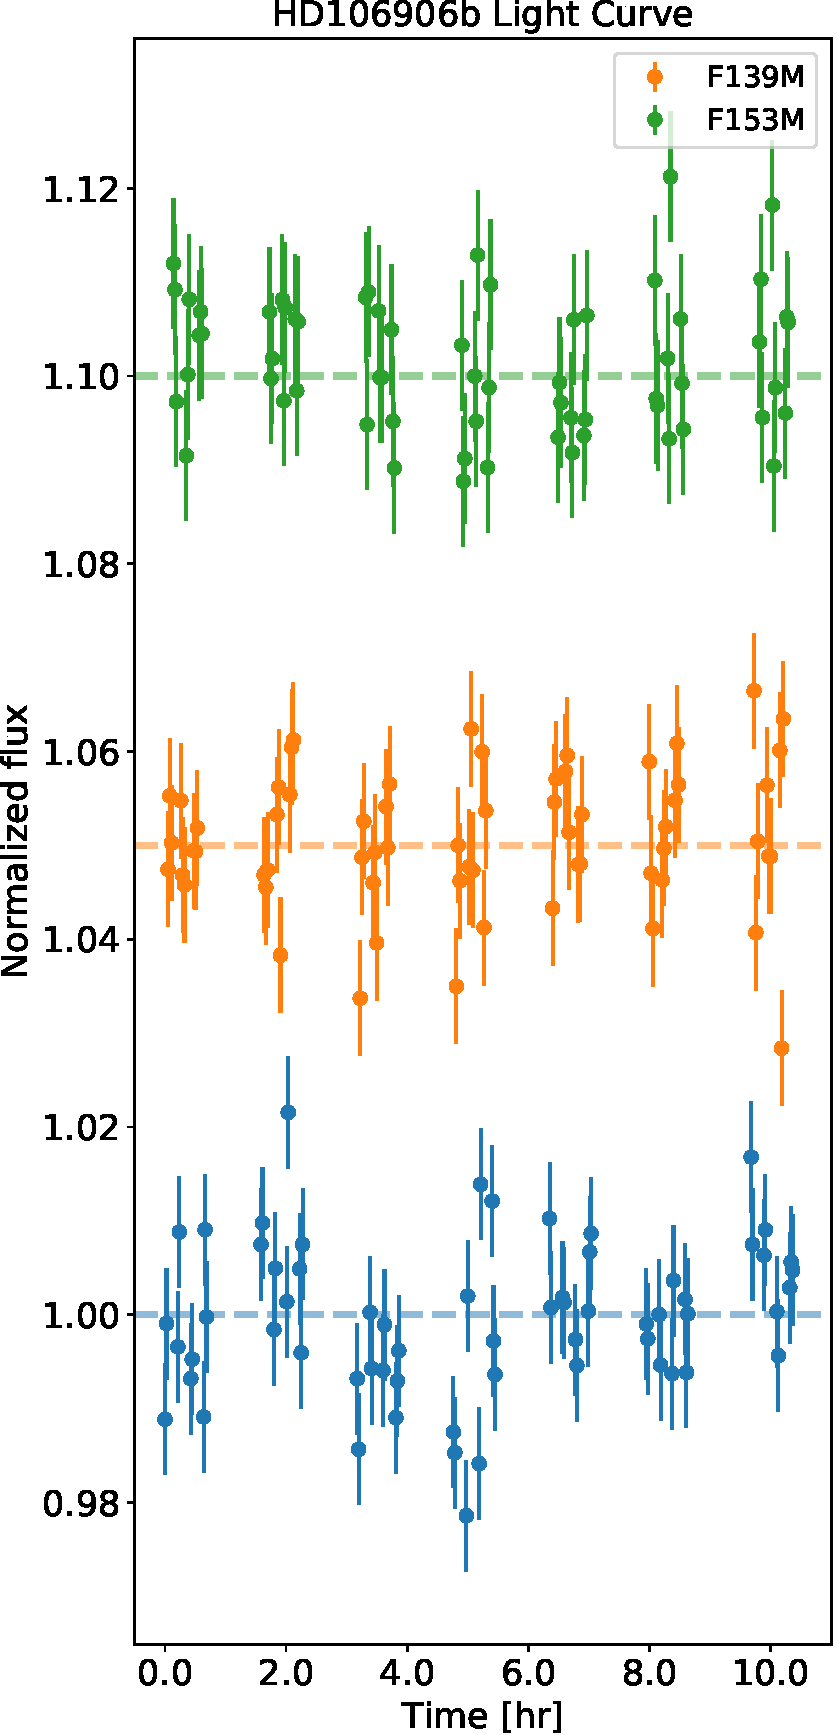
\includegraphics[width=0.5\textwidth]{figures/HD106906_lightcurves.pdf}
  \caption{The light curve for HD106906b in the F127M, F139M, and F153M}
  \label{fig:lightcurve}
\end{figure}

\begin{figure}
  \centering
  \plotone{figures/HD106906_powerspectrum.pdf}
  \plotone{figures/periodogram_bootstrap}
  \caption{Lomb-Scargle periodogram for the light curves of HD106906b.}
  \label{fig:periodogram}
\end{figure}

\begin{figure}
  \centering
  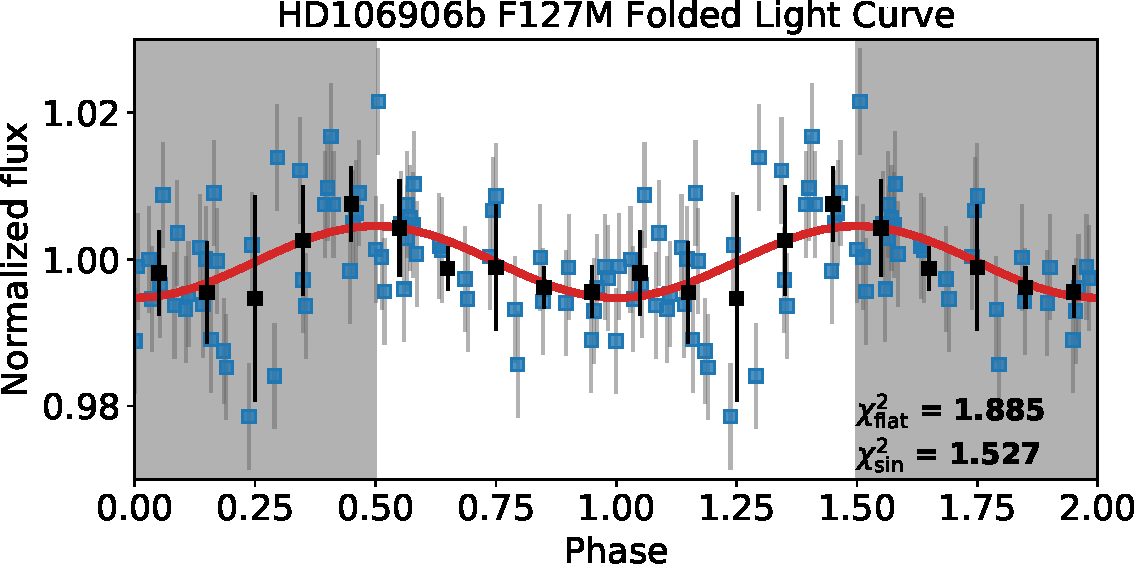
\includegraphics[width=0.5\textwidth]{figures/F127M_foldedLC.pdf}
  \caption{Phase-folded light curve for F127M. The light curve is folded to a period of 4.02 hr. The period corresponds to the most significant peak in the Lomb Scargle periodogram.}
  \label{fig:fold}
\end{figure}

\begin{figure*}
  \centering
    \plotone{figures/all-LSs}
  \caption{Comparison of the periodograms between those for background stars and those for HD106906b. The two background star periodograms that show simialr signals as HD109606b's do not show variations in the folded light curves.}
  \label{fig:all-periodograms}
\end{figure*}


\subsection{Spectral Energy Distribution}
We combine our photometry results with archival data to investigate the spectral energy distribution (SED) of HD106906b.  We use HST/ACS/F606W band photometry ($\lambda_{\mathrm{pivot}}=0.596\micron$, FWHM$=0.234\micron$) from \citet{Kalas2015}, $K_{s}$ ($\lambda_{\mathrm{pivot}}=2.145\micron$, FWHM$=0.305\micron$) and $L'$ ($\lambda_{\mathrm{pivot}}=3.774\micron$, FWHM$=0.592\micron$) band photometry from \citet{Bailey2013}. We do not use the archival $J$ band photometry because our F127M photometry characterizes similar spectral features and has more than $20\times$ greater SNR. Our F139M photometry provide a tight $1.4\micron$ water absorption constraint for HD106906b.

We fit the SED of HD106906b to the BT Settl model \citep[][Figure~\ref{fig:SED}]{Allard2012}. We perform model fitting in magnitude scale,  for which we convert the flux intensity to magnitude and linearly interpolate the model grid in magnitude scales. The free parameters are effective temperature $T_{\mathrm{eff}}$, surface gravity $\log g$, and a scaling parameter. Because model SEDs are presented as the flux at the photosphere surface, the scaling parameter can be translate to the photospheric radius. Using least $\chi^{2}$ criterion, we find the best-fitting $T_{\mathrm{eff}}=1,800\pm100$~K and $\log g=5.5\pm0.5$.  The scaling parameter corresponds to a radius of  $1.775pm0.015R_{\mathrm{Jup}}$ at a distance of 103.3~pc \citep{Gaia2018,Gaia2016}. The 1,800~K effective temperature estimate is consistent with previous study \citep{Bailey2013,Wu2016}, but the surface gravity is not compatible with a low surface gravity assessment. In addition, the model SED under-predicts the F139M band flux, or over-predicts the depth of the water absorption band.

\begin{figure*}
  \centering
  \plottwo{figures/SEDfit.pdf}{figures/SEDfit_zoomin.pdf}
  \caption{The SED of HD106906 and the best-fitting BT Settl model. The left panel shows the full observed SED (blue) that includes photometry from both this observation and archival data. The red line is the best-fitting BT Settl spectrum (1800~K, $\log g=5.5$). The red dots are the model photometry that are from model spectrum integrated with the filter throughput curves. The right panel zooms in the wavelength range of this observation. The orange violin plot shows the uncertainty of the model fitting. The flux in the F139M band is significantly under-predicted by the BT Settl model.}
  \label{fig:SED}
\end{figure*}

\subsection{Other sources in the field}
Our $30\arcsec\times30\arcsec$ field of view deep image (Figure \ref{fig:2rdi}) may include yet undiscovered companions of HD106906. In addition, the water absorption depth is an effective criterion to select ultra-cool objects. Here we define the water absorption depth as the difference between the F139M flux intensity and the continuum, which is average flux intensity of F127M and F153M. This difference is further normalized by the continuum flux to get the relative water absorption depth. The relative water absorption depth is calculated as the following equation.
\begin{equation}
D = \frac{(f_{\mathrm{F127M}} + f_\mathrm{F153M})/2 - f_{\mathrm{F139M}}}{(f_{\mathrm{F127M}} + f_\mathrm{{F153M}})/2}
\end{equation}
We used the median-combined primary-subtracted image to measure the relative water absorption depth for 12 point sources (include HD106906b) that are in the field of view for both telescope rolls. Figure~\ref{fig:backgroundsources} shows the water absorption depth for each source. Except HD106906b, there is one source that has significant water absorption depth. Interestingly, this source is the one that is discussed in \S\ref{sec:astrometry}, and also the one that has the smallest angular separation to HD106906b among all sources in the field of view. However, its astrometry is not consistent of co-moving with HD106906 but of being a background star (see \S\ref{sec:astrometry}). Based on HST/ACS/HRC and HST/WFC3/IR observation, the spectral energy distribution of the background star is best fit to a $3.7\pm0.1\times10^{3}$~K stellar SED model. Therefore, this object is most likely a background K/M giant star.

\begin{figure}
  \centering
  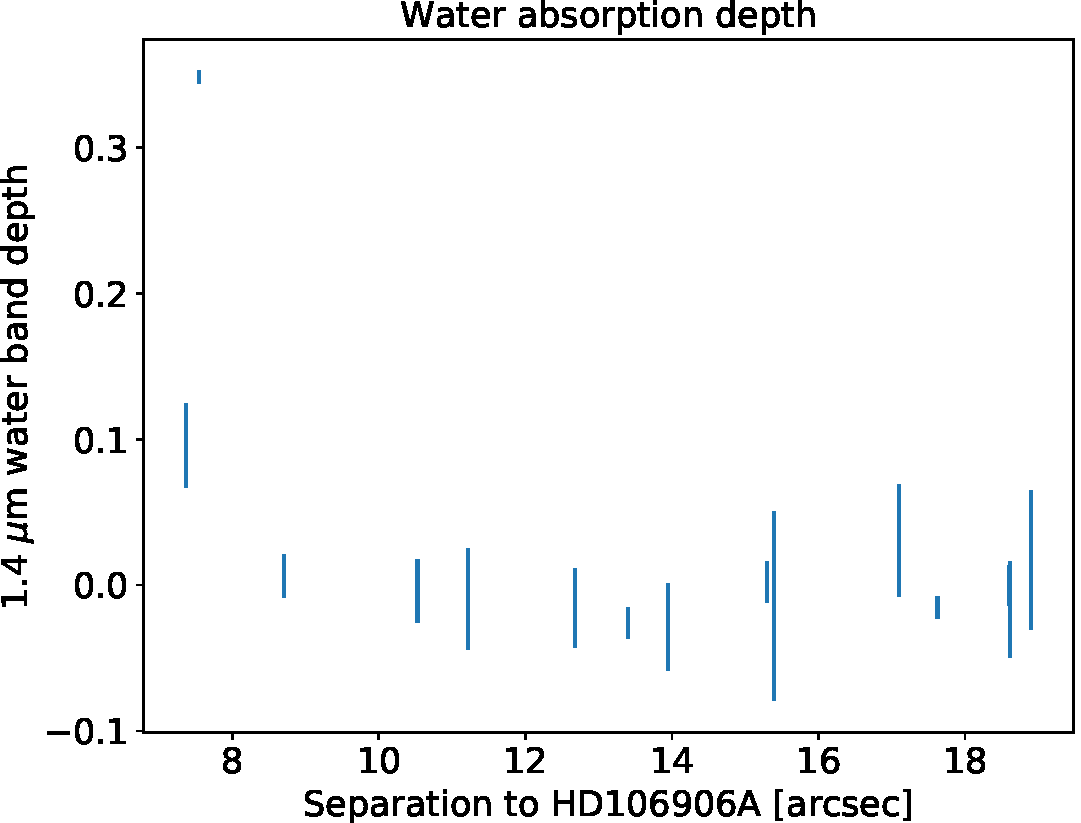
\includegraphics[width=0.5\textwidth]{figures/bck_waterdepth.pdf}
  \caption{Water absorption depths of all sources in the field of view. The sources are ranked by their angular distance to HD106906AB. The two sources (one is HD106906b) that have significant water absorption are also the two that are closest to HD106906AB in agnular distance.}
  \label{fig:backgroundsources}
\end{figure}

We calculated the 5-$\sigma$ contrast curves for the median-combined primary-subtracted images in all three bands (Figure \ref{fig:contrast_curve}). The method of constructing these contrast curves through a PSF injection-and-recovery process, which is detailed in  \citet{Zhou2019}.  We found that the three bands: F127M, F139M, and F153M have almost the same contrast curves and the F127M image has the contrast at large separation. The similarity of the contrast curve is due to that the brightness of HD106906 is almost identical in these three bands and the F127M brightness is slightly higher than the other two bands. Our median-combined, primary-subtracted images are sensitive to $\Delta \mbox{mag}=7.7$ at 1\arcsec, $\Delta \mbox{mag}=10.4$ at 2\arcsec, and $\Delta \mbox{mag}=14.2$ at 5\arcsec. Assuming an age of 15 Myr and evolution track of \citet{Saumon}, our median-combined, primary-subtracted images can place 5-$\sigma$ upper limits for companions more massive than 7\mjup at 2\arcsec or wider and 2\mjup at 4.75\arcsec or wider.

\begin{figure}
  \centering
  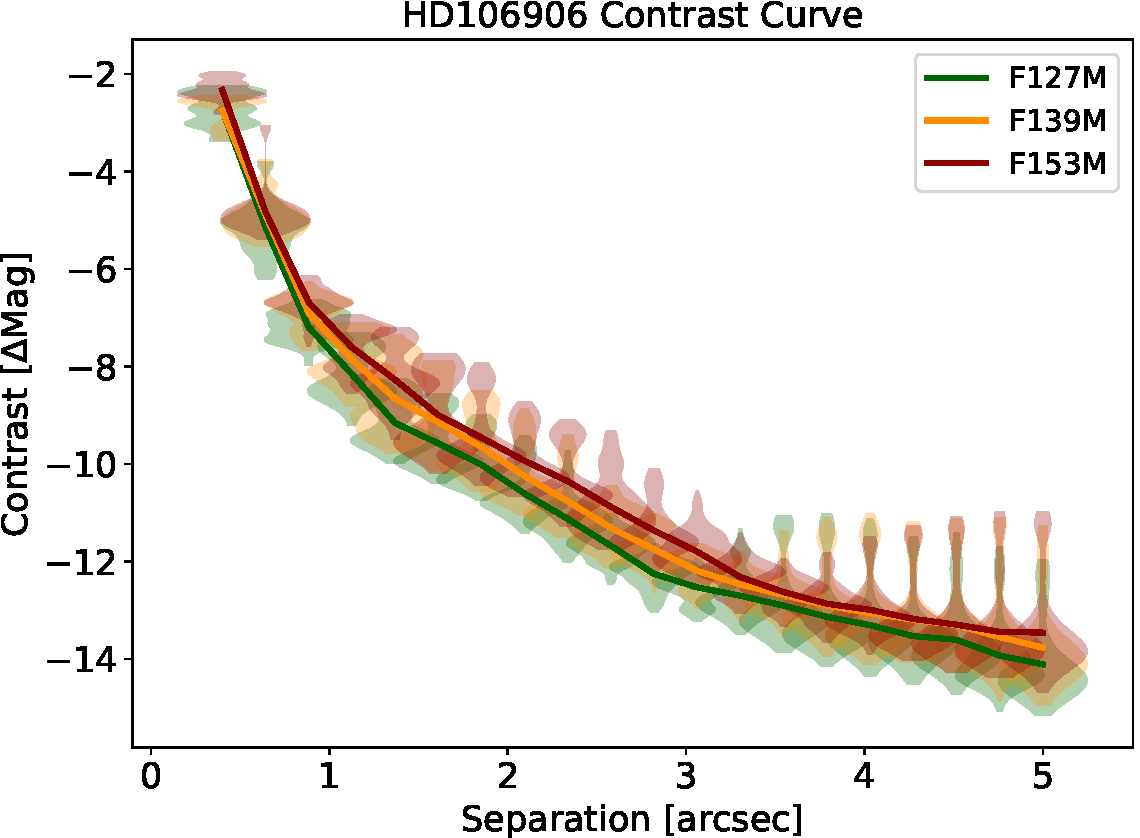
\includegraphics[width=0.5\textwidth]{figures/contrast_curve.pdf}
  \caption{Contrast curves in F127M, F139M, and F153M for the HD106906 observations.}
  \label{fig:contrast_curve}
\end{figure}

\subsection{Astrometry -- orbital motion of HD106906b}
TO BE IMPLEMENTED

\subsection{Astrometry -- relative to the background star}
\label{sec:astrometry}
We are particularly interested in the background star that is only 0\arcsec{}.87 away from HD106906b. It is unreported in previous studies and could contaminate the photometric and spectroscopic observations of HD106906b.  We calculate the differences in right ascension ($\Delta$RA),  declination ($\Delta$DEC), and the separations between HD106906b and the background star from year 2003 (one year before the first direct imaging record of HD106906b) to year 2023. In this calculation, the background star is assumed to be stationary and HD106906b is co-moving with its host star at $(\mu_\alpha\cos\delta=-39.01 \mbox{mas/yr}, \mu_{\delta}=-12.87 \mbox{mas/yr})$ \citep{Gaia2016, Gaia2018}. The results are shown in Figure~\ref{fig:astrometry:bck}. In the same figures, we also marked the previous observations \citep{Bailey2013, Wu2016, Lagrange2016, Daemgen2017} to evaluate if the background star was detectable or could contaminate the measurements in those observations.

Figure~\ref{fig:astrometry:bck} demonstrates that HD106906b, due to its proper motion, has been approaching  the background star over the years. The separation between these two object has shortened from 1\arcsec.29 (2004, first imaging record) to 0\arcsec.87 (this study). In the study of \citep{Bailey2013, Wu2016, Daemgen2017}, the background star had separation of 0.95-1.05 to HD106906b. Given their separations in these studies, it is unclear if the background star contaminated those measurements. Considering the brightness contrast of the two object, in the worst case, the contamination of the background star to HD106906b's broadband photometry is  $<7.5\%$ in the near-infrared.

\begin{figure*}
  \centering
  \plottwo{figures/bckStarDeltaRADEC.pdf}{figures/bckStarSeparation.pdf}
  \caption{Relative astrometry between HD106906b and a closeby background star. Left: The difference in right ascension and declination. Right: The separation as a function of time. Past observations of HD106906b are marked as squares.}
  \label{fig:astrometry:bck}
\end{figure*}


% \Interestingly{Large scale structures}


\section{Discussion}
\subsection{Light curve periodicity}

We evaluate the modulation significance in both instrumental and astrophysical perspective. From the instrumental point of view, we have two arguments against that the modulation signal we see in HD106906b's F127M light curve is due to systematics. First, the F127M, F139M, and F153M observations were taken \emph{de facto} simultaneously. Systematics that introduces periodic/sinusoidal signals at 4 hr timescale in the F127M light curve should have similar effect on the other two light curves. Agreement between F139M and F153M light curves with flat lines is inconsistent with modulation in the F127M light curve being systematics. Second, similar modulations do not appear in the light curves of background stars. We measure and analysis light curves of fifteen brightest background stars that are in the field of view of both telescope roll angles and are not affected by the diffraction spikes of the primary PSFs. In the appendix we list the light curves and periodograms for all background stars. Figure \ref{fig:all-periodograms} shows the comparison between the periodograms of the background stars and that for F127M light curve of HD106906b. Most periodogram of the background star do not show significant signals except one object. However, when we fold its light curve to the period with the most significant peak, the folded light curve is consistent with a flat line. These two lines of evidence argue that systematics is not likely to be the cause of the modulation signal.

From astrophysical perspective, we evaluate the likelihood for HD106906b to be rotationally modulated only in the F127M band but not the other two bands. Multi-wavelength and time-resolved observations of ultra-cool dwarfs have found the rotational modulations for majority  brown dwarfs and planetary mass companions are spectrally dependent and have greater amplitude at shorter wavelengths than longer wavelengths \citep[e.g.,][]{Zhou2019,Zhou2016,Yang2014,Apai2013,Schlawin}. This phenomenon is consistent with theoretical estimation based on Mie-scattering calculation\citep{Schlawin,Hiranaka2016}. In addition, the 1.4 \micron{} water absorption/F139M band often show damped rotational modulation, due to water vapor opacity elevating the photosphere at this wavelength.  Therefore rotational modulation only appearing in the bluest band of our observation is qualitatively consistent with theoretical model and previous observations, particularly those for planetary mass companions \citep{Zhou2016,Zhou2019}. If we assume that the wavelength dependence of HD106906b's rotational modulation is the same as that measured in 2M1207b \citep{Zhou2016}, as 2M1207b is the closest analogue that also has modulation detected, a 0.49\% modulation in the F127M band should correspond to a 0.06\% modulation in the F153M band. Such a small amplitude is below the sensitivity of our observation. Therefore, if the overall modulation amplitude is small, it is likely that the signal is only detected in the bluest band of the observation.

These two lines of evidence support the modulation we see in HD106906b's F127M light curve to be astrophysical origin, in particular, caused by heterogeneous clouds. Nevertheless, we emphasize that the amplitude of the signal is small and marginally detected. Our evaluation on the rotational modulation and rotation period for HD106906b remain inconclusive.


\subsection{SED of  HD106906b}
Two issues have emerged in the SED fitting results. First, the best-fitting model over-predicts the 1.4 \micron{} water absorption band depth. Second, the best-fitting surface gravity is inconsistent with previous low-gravity assessment for HD106906b.

To investigate the first issue, we calculate the water band absorption depths in the BT Settl as functions of $T_{\mathrm{eff}}$ and $\log g$ and compare them with the observed value. As shown in Figure \ref{fig:waterdepth}), for a fixed $T_{\mathrm{eff}}$ of 1800 K, all BT Settl models over-predict the water band depth. For a fixed $\log g$ of 5.5, to match the observed water band depth, $T_{\mathrm{eff}}$ needs to be raised to $2500$ K, although such a high temperature is not at all consistent with the overall SED shape. Therefore, the mismatch between the HD106906b's observed and the model SEDs in the 1.4 \micron{} water bands demonstrates the inadequacy of current state-of-the-art ultra-cool atmospheric models.

\citet{Bailey2013} and \citet{Daemgen2017} have discussed the surface gravity of HD106906b. Both studies classify HD106906b as a low-to-intermediate surface gravity object based on its triangle-shaped $H$ band spectrum. The equivalent widths of the K I absorption lines measured in \citet{Daemgen2017} are also consistent with an intermediate surface gravity classification. In addition, low surface gravity is also consistent with the young and low mass nature of HD106906b. However, our SED fitting yield a very high gravity result. With a fixed $T_{\mathrm{eff}}$ of 1800 K, lower surface gravity models significantly over-predicts the F153M and $K_{\mathrm{s}}$ band flux intensities, therefore they are not preferred by the SED fitting. This inconsistency, again, may show the insufficiency of atmospheric models for planetary-mass ultra-cool objects.

\begin{figure}
  \centering
  \plotone{figures/logg_water}
  \plotone{figures/Teff_water}
  \caption{1.4 \micron{} water band depths predicted by the BT Settl model. Left: With a fixed $T_{\mathrm{eff}}=1800$ K, models with $\log g$ between 3 to 5.5 all over-predicts the water band depths. Right: With a fixed $\log g=5.5$, it requires $T_{\mathrm{eff}}=2500$ K for the model to match the observation.}
  \label{fig:waterdepth}
\end{figure}

\subsection{Orbit and dynamical evolution of the HD106906 system}


\section{Conclusion}

\begin{enumerate}
\item We observed planetary mass companion HD106906b with seven contiguous HST orbits in HST WFC3/IR direct-imaging mode. We have achieved photon-noise limited sub-percent level precision light curves in F127M, F139M and F153M bands. Rotational modulations marginally ($2-\sigma$) presents in the F127M band but are absent in other two bands.

\item Comparing to planetary mass companions that have time-resolved observations, the marginal detection of  F127M band modulations and non-detections in other two bands are consistent with those brown dwarfs and planetary mass companions for which the rotational modulations are detected at high significance. The wavelength-dependent rotational modulations are consistent with the interpretation that the modulations are caused by heterogeneous condensate clouds.

\item Our observations provide the first 1.4 \micron water band photometry for HD106906b. We combine our three bands of photometry with archival data to form a SED for HD106906b and perform SED model fitting. We find a best-fitting effective temperature of 1800~K, consistent with literature results, and a best-fitting surface gravity $\log g$ of 5.5,  significantly higher than previous estimate and inconsistent with HD106906b being a young and planetary mass object. In addition, the observed F139M band flux intensity for HD106906b is significantly higher than the best-fitting model value. These inconsistency may suggest inadequacy of the BT-Settl model for young planetary mass objects.

\item We combine WFC3/IR images to form primary-subtracted deep imaages and search for new planetary mass companions in the field of view. Our composite images are sensitive to planet with a mass of $\sim 2 \mjup$. We used the 1.4mm water absorption to further vet the companions. We did not discover  any new companions. We did find a point source that have lower flux in the F139M band. This object is likely a background K/M giant due to its bluer color and consistence with stationary astrometry location.

\item The object that has apparent water absorption happened to be in close proximity to HD106906b. Based on GAIA astrometry and proper motion, the angular distance between HD106906b and the background star is decreasing and will be on the level of 0\arcsec.7-0\arcsec.8  in the coming decade. Future observations of HD106906b needs to carefully eliminate contamination from the background star.

\item Astrometry related discussion:  orbit and dynamic evolution.
\end{enumerate}
% \end{enumerate}
% For the last point, take the variability occurrence rate from \citep{Vos2017,Metchev2015}, test whether the low mass companions' variability occurrence rate agree with the low surface gravity field objects
\bibliographystyle{yahapj}
\bibliography{library}

\end{document}
%%% Local Variables:
%%% mode: latex
%%% TeX-master: t
%%% End:

% LocalWords:  AAS
